%==============================================================================
% CAPITOLUL 4 - Testarea si evaluarea sistemului
% Se adauga in continuarea Capitolului 3.
% Redactat cu diacritice, conform Regulamentului ETTI (Cap. 3).
%==============================================================================

\chapter{Testarea și evaluarea sistemului}
\label{cap:testare}

După implementarea funcționalităților și punerea în funcțiune a platformei,
descrise în capitolele anterioare, etapa următoare a constat în testarea
sistemului pentru a verifica funcționarea corectă a fiecărei componente și
comportamentul de ansamblu al aplicației în condiții reale de utilizare. Acest
capitol descrie metodologia de testare adoptată, scenariile parcurse, rezultatele
observate și limitările identificate. Scopul este de a oferi o evaluare onestă a
platformei în starea sa actuală, evidențiind atât aspectele care funcționează
conform așteptărilor, cât și pe cele care reprezintă oportunități de îmbunătățire
ulterioară.

\section{Metodologia de testare}
\label{sec:metodologie-testare}

Pentru evaluarea platformei ETTIway am adoptat o abordare de testare
preponderent manuală, orientată spre scenarii reale de utilizare. Această alegere
este motivată de natura aplicației: ETTIway este o platformă cu o componentă
vizuală și interactivă semnificativă, iar comportamentul său în condiții reale
(recepția GPS în campus, fluiditatea interacțiunii cu harta sau
claritatea afișării) nu poate fi evaluat automat, ci necesită observare directă
pe dispozitivele țintă.


Testarea am desfășurat-o pe două direcții complementare. Prima direcție a vizat
verificarea funcțională a fiecărei capabilități în parte. Autentificarea în cele
două roluri, căutarea unei săli, afișarea detaliilor, editarea hărții de către
administrator, persistarea modificărilor în baza de date și calculul traseului
între două puncte. A doua direcție a vizat verificarea de ansamblu a fluxului de
utilizare, parcurgând scenariile complete de la deschiderea aplicației până la
afișarea unui traseu pe hartă, pentru a observa modul în care componentele
conlucrează.


\section{Scenarii de testare funcțională}
\label{sec:scenarii}

Funcționalitățile centrale ale platformei au fost verificate sistematic, prin
parcurgerea unor scenarii reprezentative pentru utilizarea reală. Această
secțiune descrie scenariile principale și rezultatele observate.

\subsection{Autentificarea și diferențierea rolurilor}
\label{subsec:test-auth}

Pentru verificarea mecanismului de autentificare, s-au parcurs scenarii cu ambele
roluri configurate: utilizator obișnuit și administrator. La introducerea
credențialelor valide, sistemul redirecționează utilizatorul către interfața
corespunzătoare rolului său, încărcând setul de controale adecvat. La
introducerea unor credențiale eronate, accesul este refuzat, iar utilizatorul
este readus la pagina de autentificare, fără a primi informații care ar putea
ajuta la identificarea cauzei refuzului, un aspect important din punct de vedere
al securității.

\newpage

Am verificat, de asemenea, izolarea funcționalităților rezervate
administratorului. Încercarea de a accesa direct, prin manipularea adresei,
rutele administrative din contul unui utilizator obișnuit este blocată la
nivelul backend-ului, confirmând că diferențierea rolurilor nu se bazează doar pe
ascunderea controalelor în interfață, ci este aplicată efectiv la nivelul
serviciilor. Această dublă protecție, în interfață și în backend, corespunde
practicilor uzuale de securizare a aplicațiilor web.


\begin{figure}[H]
    \centering
    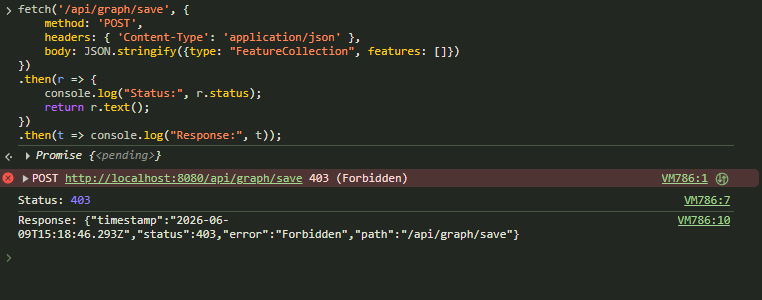
\includegraphics[width=0.8\textwidth]{figuri/mesaj_consola.png}
    \caption{Mesaj afișat în consola la încercarea de salvare a hărții de un cont de user obișnuit}
    \label{fig:mesaj-consola}
\end{figure}

\subsection{Căutarea și afișarea detaliilor}
\label{subsec:test-cautare}

Funcția de căutare am evaluat-o prin introducerea unor termeni
reprezentativi, nume de clădiri și de săli din campus, și observarea
rezultatelor afișate. Am verificat atât potrivirile exacte, cât și
potrivirile parțiale, pentru a confirma că aplicația găsește elementele corecte
chiar și atunci când utilizatorul introduce doar o parte a denumirii. La
selectarea unui rezultat, detaliile asociate, clădirea, etajul, capacitatea,
tipul, sunt afișate complet și consistent, atât în panoul lateral, cât și în
ferestrele de tip pop-up atașate locațiilor pe hartă.



\subsection{Editarea și persistența modificărilor}
\label{subsec:test-editare}

Pentru rolul de administrator, am verificat ciclul complet de editare a
hărții: autentificare ca administrator, intrarea în modul de editare, adăugarea
și modificarea unor noduri și legături, salvarea modificărilor și verificarea
menținerii acestora în baza de date. Modificările sunt vizibile imediat după salvare, iar
reîncărcarea aplicației, chiar și de pe alt dispozitiv, confirmă faptul că noile date
sunt preluate corect din baza de date și prezentate consistent tuturor
utilizatorilor. Acest scenariu confirmă funcționarea fluxului complet între
frontend și backend.



\subsection{Calculul și afișarea traseului}
\label{subsec:test-traseu}

Componenta de rutare am evaluat-o prin selectarea unor perechi de puncte
distribuite în campus și verificarea traseelor calculate. În toate cazurile în
care punctele se află pe porțiuni conectate ale rețelei, algoritmul returnează un
traseu, iar acesta este desenat clar pe hartă, urmărind rețeaua de alei și
drumuri. Pentru cazurile particulare, punct de plecare identic cu cel de
destinație, puncte foarte apropiate, puncte aflate pe componente neconectate ale
grafului, am verificat comportamentul aplicației, aceasta tratând corect
fiecare situație, fie prin afișarea unui traseu degenerat la un singur punct, fie
prin semnalarea absenței unui drum.

\subsection{Editarea și rutarea în interior}
\label{subsec:test-indoor}

Componenta de rutare indoor am verificat-o folosind date reale: o clădire
din campus, pentru care administratorul a desenat planul unui etaj cu mai multe
camere, un set de coridoare conectate prin intersecții și nodurile de intrare
asociate fiecărei camere. Am parcurs, pe rând, cele două roluri ale
fluxului indoor.

Pentru rolul de administrator, am verificat ciclul complet de editare:
desenarea camerelor cu introducerea numelui, plasarea markerilor cu alegerea
tipului (intrare cameră, intersecție sau scară), trasarea coridoarelor între
markeri și salvarea planului. La reîncărcarea aplicației, planul a fost
încărcat corect din baza de date, incluzând proprietățile fiecărui element și
ferestrele de tip tooltip atașate camerelor.

Pentru rolul de utilizator obișnuit, am verificat fluxul de căutare și
rutare. Căutarea unei camere a deschis automat planul etajului corespunzător,
cu camera țintă evidențiată vizual. Selectarea unui punct de plecare din
lista de noduri disponibile și apăsarea butonului de calcul al traseului a
condus la afișarea drumului optim între punctele alese, urmărind rețeaua de
coridoare. Mecanismul de proiectare a nodurilor pe segmente apropiate, descris
în Capitolul~3, s-a dovedit util în practică: micile imprecizii din desen, în
care o linie nu se conectează exact la un alt segment, sunt tolerate fără a
afecta calculul traseului.

Cazul particular al rutării între etaje diferite, neimplementat în versiunea
actuală, este tratat explicit de aplicație printr-un mesaj informativ pentru
utilizator, evitând rezultate inconsistente.

\section{Testarea pe mai multe dispozitive și browsere}
\label{sec:portabilitate}

Deoarece ETTIway este o aplicație web, o cerință importantă este funcționarea
corectă pe o varietate de dispozitive și de browsere. Testarea a inclus accesarea
aplicației de pe calculatoare personale, prin browserele cele mai răspândite,
precum și de pe telefoane mobile cu sisteme de operare diferite. În toate
configurațiile testate, aplicația s-a comportat uniform: harta s-a încărcat
corect, controalele au răspuns natural la interacțiune, iar funcționalitățile de
căutare și rutare au funcționat identic.

Această consistență confirmă alegerea tehnologică de a folosi exclusiv API-uri
web standard, fără dependențe de capabilități specifice unui anumit browser.
Suportul nativ oferit de biblioteca Leaflet pentru gesturile tactile
(deplasarea hărții prin glisare, mărirea prin apropierea degetelor) a contribuit
semnificativ la o experiență fluidă pe dispozitivele mobile, care reprezintă
contextul principal de utilizare a platformei într-un campus.

\section{Comportamentul în condiții reale de utilizare}
\label{sec:conditii-reale}
 
Pe lângă scenariile individuale de testare, am folosit aplicația în
condiții reale, parcurgând efectiv campusul cu un dispozitiv mobil pe care rula
aplicația. Acest tip de evaluare, dificil de înlocuit prin teste automate, a
oferit informații valoroase despre comportamentul de ansamblu și despre
experiența reală a utilizatorului.
 
În spațiile deschise, în care recepția GPS este bună, poziția utilizatorului
afișată pe hartă urmărește fidel deplasarea reală, iar traseele calculate către
diferite destinații sunt afișate fluid, în timp real. Tranziția între pașii
fluxului de utilizare, autentificare, alegerea destinației, calculul traseului,
afișarea sa pe hartă, se desfășoară fără întreruperi vizibile, iar timpul de
răspuns al aplicației nu a constituit, în testele efectuate, un factor limitativ.
 
Trecerea de la spațiul exterior la interiorul unei clădiri, deși nu este
tratată automat în versiunea actuală, se face cu o experiență fluidă din
perspectiva utilizatorului: o singură interacțiune (deschiderea planului
clădirii dorite) marchează tranziția între cele două moduri de navigare, iar
contextul vizual al hărții exterioare este păstrat în fundal, oferind un
sentiment de continuitate.
 
În contextul utilizării prin rețeaua privată Tailscale, latența suplimentară
introdusă de criptarea VPN și de tranzitul prin serverele de coordonare nu a
fost perceptibilă pentru utilizator. Comparativ cu accesarea aplicației
direct, prin rețeaua locală, diferențele de timp de răspuns au fost de ordinul
zecilor de milisecunde, sub pragul de percepție umană pentru interacțiunile
cu o interfață web.

% [SUGESTIE CAPTURA 4.3: captura de pe telefon facuta in campus, in aer liber,
% aratand pozitia utilizatorului pe harta si traseul calculat. Plaseaz-o aici.]

\section{Limitări identificate}
\label{sec:limitari}

Testarea sistematică și utilizarea în condiții reale au evidențiat și anumite
limitări, care merită discutate atât pentru completitudinea evaluării, cât și
pentru a identifica direcțiile naturale de dezvoltare ulterioară.

\subsection{Precizia poziționării în interiorul clădirilor}
\label{subsec:limitare-gps}

Limitarea cea mai vizibilă în utilizarea reală este legată de precizia
poziționării atunci când utilizatorul se află în interiorul clădirilor. În
spațiile deschise, semnalul GPS oferă o precizie de ordinul câtorva metri,
suficientă pentru a indica corect poziția pe rețeaua de alei a campusului. În
interiorul clădirilor, însă, semnalul satelitar este atenuat și reflectat de
structurile de beton și metal, ceea ce conduce la o degradare semnificativă a
preciziei, eroarea putând ajunge la zeci de metri.

\begin{table}[htbp]
    \centering
    \caption{Precizia GPS măsurată în diferite contexte de testare}
    \label{tab:precizie-gps}
    \begin{tabular}{lcc}
        \toprule
        \textbf{Locație testare} & \textbf{Precizie raportată (m)} & \textbf{Observații} \\
        \midrule
        Curtea ETTI (spațiu deschis)          & 4-8        & Funcționare optimă \\
        Aleea principală campus               & 5-10       & Precizie acceptabilă \\
        Lângă corpul A (clădire înaltă)       & 10-20      & Multipath vizibil \\
        Intrare corp B                        & 15-25      & Tranziție exterior-interior \\
        Hol corp B (interior)                 & 30-50      & Eroare semnificativă \\
        Sală de curs (interior adânc)         & 50-100+    & Practic inutilizabil \\
        \bottomrule
    \end{tabular}
\end{table}


Această limitare nu este specifică implementării ETTIway, ci este o caracteristică
fundamentală a tehnologiei GPS, întâlnită în orice aplicație care depinde de
poziționarea satelitară. Ea a fost descrisă, din punct de vedere teoretic, în
Capitolul 1, iar testarea practică a confirmat efectul observat și anticipat:
funcționarea optimă a localizării este în spațiu deschis, ceea ce corespunde și
contextului principal de utilizare a unei aplicații de navigare în campus,
adică deplasarea între clădiri, pe alei. Pentru orientarea în interiorul clădirilor,
soluții complementare, bazate pe alte tehnologii de localizare, ar putea fi
integrate în versiuni viitoare, aspect discutat în capitolul de concluzii.

\subsection{Acoperirea actuală a datelor}
\label{subsec:limitare-date}

O a doua limitare, distinctă de cea tehnologică, ține de gradul actual de
completitudine a datelor introduse în platformă. Aplicația funcționează corect în
măsura în care harta și rețeaua de trasee acoperă fidel infrastructura
campusului. Extinderea acoperirii, adăugarea de noi clădiri, alei sau puncte de
interes, este însă posibilă direct, prin intermediul modului de editare
descris în capitolul anterior, fără modificări în cod. Această proprietate face
ca limitarea să fie una de scop, nu una structurală, și să poată fi depășită prin
muncă incrementală de întreținere a datelor.

\section{Concluziile capitolului}
\label{sec:concluzii-cap4}

În acest capitol au fost prezentate metodologia, scenariile și rezultatele
testării platformei ETTIway. Funcționalitățile principale, autentificarea cu
diferențierea rolurilor, căutarea, afișarea detaliilor, editarea hărții cu
persistarea modificărilor și calculul vizual al traseelor, au fost verificate
sistematic, prin scenarii reprezentative, și au fost confirmate ca funcționând
conform așteptărilor. Testarea pe mai multe dispozitive și browsere a arătat un
comportament uniform, validând alegerile tehnologice care favorizează
portabilitatea.

Evaluarea în condiții reale, prin utilizarea aplicației în campus, a confirmat că
experiența de navigare este fluidă în spațiile deschise, în care recepția GPS
este bună. Singura limitare semnificativă identificată este degradarea preciziei
poziționării în interiorul clădirilor, o caracteristică intrinsecă a tehnologiei
GPS, care delimitează în mod natural domeniul de utilizare optimă a aplicației la
navigarea în spațiile exterioare ale campusului. Această observație, formulată
explicit, oferă o bază clară pentru direcțiile de dezvoltare ulterioară, discutate
în concluziile finale ale lucrării.


\begin{figure}[H]
    \centering
    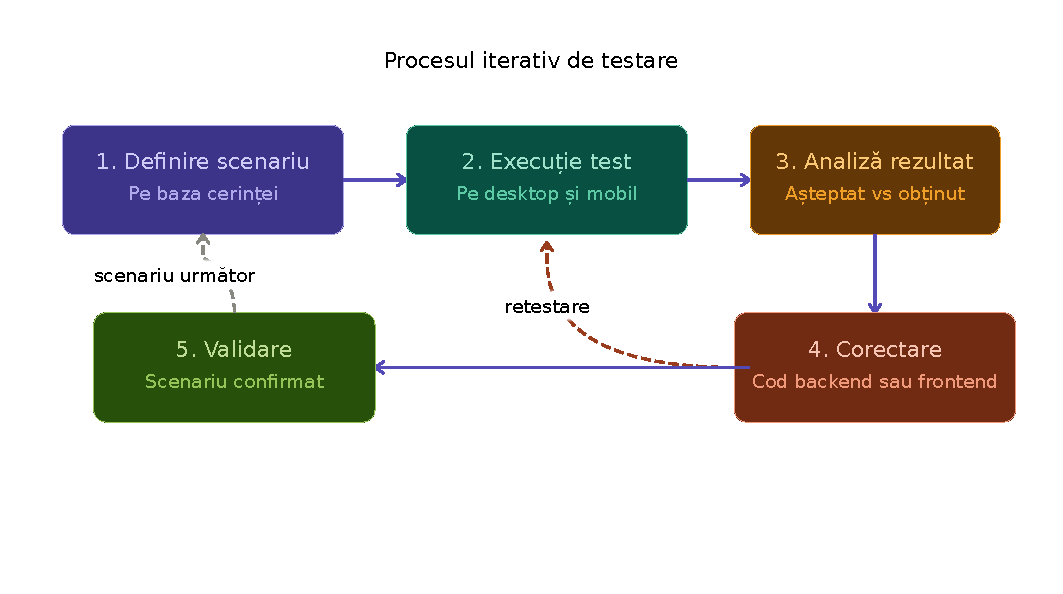
\includegraphics[width=1\textwidth]{figuri/flux_testare.pdf}
    \caption{Diagrama fluxului de testare a platformei }
    \label{fig:flux-auth}
\end{figure}